\section{Method}\label{method}

This study proposes a reusable local benchmarking pipeline for selecting embedding models under corpus-specific Retrieval-Augmented Generation (RAG) requirements. The method is organized as a staged workflow that transforms local document collections into controlled benchmark artifacts, including chunked corpora, synthetic queries, relevance judgments, model-specific vector indexes, and structured reporting outputs. Each intermediate artifact serves as a controlled input to the next stage, which allows candidate embedding models to be evaluated under the same benchmark evidence rather than under model-specific or manually curated test sets. This design supports both single-dataset model selection and, when heterogeneous corpus subsets are benchmarked separately, aggregate comparison across topic- or language-specific dataset partitions.

\subsection{Pipeline Overview}\label{pipeline-overview}

The pipeline operates at the dataset level and begins with explicit dataset routing, as illustrated in Figure~\ref{fig:method_pipeline_workflow}. Each corpus is processed in isolation so that document inputs, chunked corpora, synthetic queries, qrels, vector collections, and reports remain separated across datasets. This design reduces cross-dataset contamination and allows the same methodological template to be applied repeatedly to document collections that differ in language, domain, and scale. After routing, the workflow advances through document ingestion, chunking, query generation, and relevance construction, thereby producing the benchmark artifacts required for comparative retrieval.

Once these shared artifacts have been created, the pipeline branches into model-specific indexing and evaluation. Separate vector collections are built for each candidate embedding model, and each model is evaluated against the same query and qrels resources rather than against model-specific or manually curated evidence. The final stage consolidates the resulting outputs into dataset-level reports and, when multiple corpora are available, into an aggregate comparison report. The sequence of stages and their intermediate products are summarized in Table~\ref{tbl:method_pipeline_stages} and illustrated conceptually in Figure~\ref{fig:method_pipeline_workflow}.

\begin{table}[t]
\caption{Stage sequence and intermediate artifacts of the proposed embedding benchmarking workflow.}\label{tbl:method_pipeline_stages}
\centering
\small
\begin{tabular}{@{}>{\raggedright\arraybackslash}p{0.14\linewidth}>{\raggedright\arraybackslash}p{0.16\linewidth}>{\raggedright\arraybackslash}p{0.38\linewidth}>{\raggedright\arraybackslash}p{0.22\linewidth}@{}}
\toprule
Stage & Input & Process & Output \\
\midrule
Dataset routing & Local dataset selection & Bind one dataset to isolated working paths so downstream artifacts remain separated across corpora & Dataset-specific run context \\
Document ingestion & Routed document collection & Parse source documents and normalize extracted text for downstream processing & Textual corpus \\
Chunking & Textual corpus & Segment documents into overlapping units suitable for embedding and retrieval & Chunked corpus \\
Query generation & Chunked corpus & Sample seed chunks and generate natural-language queries in the source language of the seed content & Synthetic query set \\
Relevance construction & Query set and chunked corpus & Retrieve a bounded candidate pool for each query and assign binary relevance labels through LLM-assisted judgment & Qrels resource \\
Multi-model indexing & Chunked corpus and selected embedding models & Build a separate vector collection for each embedding model so retrieval runs remain isolated and reproducible & Per-model vector collections \\
Retrieval evaluation & Query set, qrels, and per-model collections & Execute the same fixed-depth retrieval workflow for every model over the same benchmark artifacts & Ranking artifacts and timing traces \\
Reporting & Dataset-level evaluation artifacts & Produce dataset-level reports and aggregate comparison artifacts for downstream interpretation & Benchmark reports and visual summaries \\
\bottomrule
\end{tabular}
\end{table}

\begin{figure}
\centering
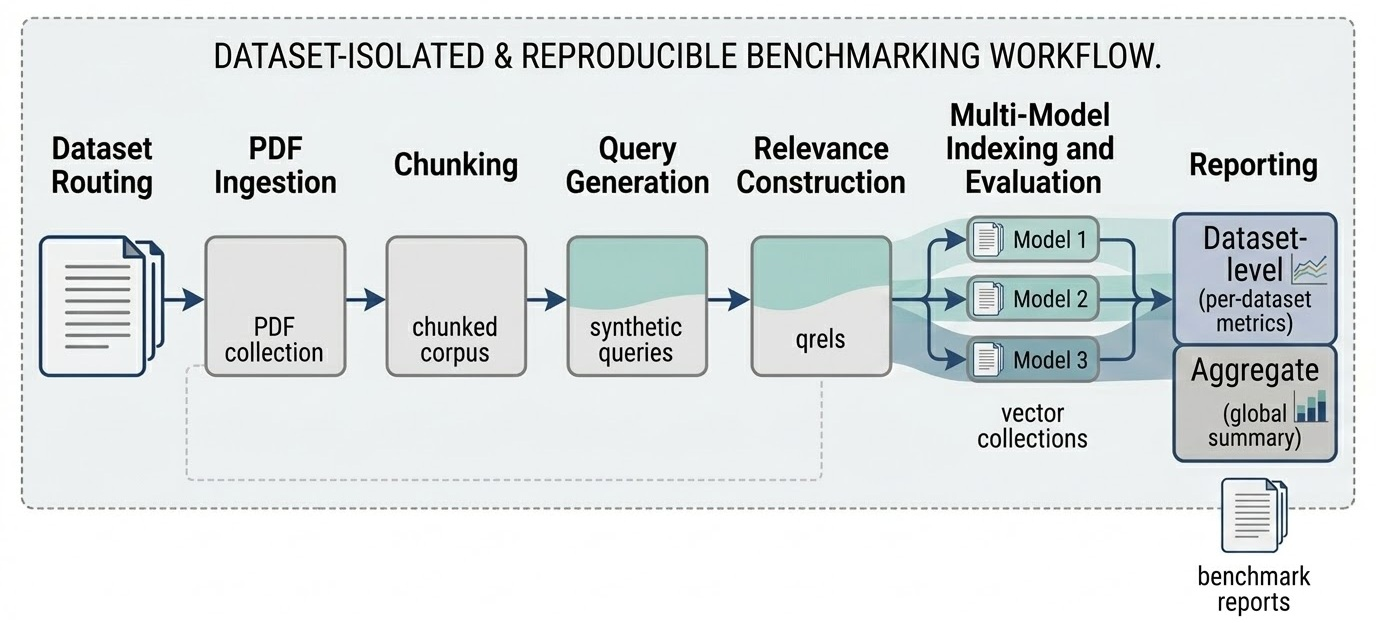
\includegraphics[width=0.95\linewidth]{conceptual_overview.jpg}
\caption{Conceptual overview of the proposed embedding benchmarking pipeline.}\label{fig:method_pipeline_workflow}
\end{figure}

\subsection{Corpus Preparation}\label{corpus-preparation}

The first stage converts each local document collection into a benchmarkable text corpus. Source documents are ingested from the local corpus and parsed into textual segments; in the present experimental snapshot, these source documents are provided as PDF files. To preserve local context while keeping units manageable for downstream embedding models, the extracted text is segmented by recursive character-based chunking with controlled overlap between adjacent segments. This strategy reduces the probability that semantically dependent passages are split into entirely disconnected units, while still producing retrieval items that can be embedded and indexed efficiently. The fixed parameterization used in the experimental instantiation of this workflow is summarized in Section~\ref{shared-evaluation-setup}.

Dataset-level isolation is maintained during corpus preparation. Each dataset yields its own chunked corpus and retains its own storage path for downstream artifacts. As a result, the same pipeline can be reused across multiple corpora without mixing documents, collections, or reports between experiments.

\subsection{Synthetic Query and Relevance Construction}\label{synthetic-query-and-relevance-construction}

After corpus construction, the pipeline constructs benchmark queries and relevance judgments through the sequence shown in Figure~\ref{fig:method_qrels_workflow}. Each instance begins with a seed chunk sampled from the corpus. Rather than relying on externally authored questions, the method prompts a large language model to generate a concise natural-language query in the same language as that sampled chunk. In this sense, the pipeline uses the language model as a query-construction judge that converts one corpus-grounded seed passage into one evaluation query while preserving the linguistic and topical characteristics of the underlying dataset. This design keeps query formulation anchored to the target corpus while avoiding the cost of manually preparing a query set for each new dataset.

Relevance construction then proceeds from the generated query. The system retrieves a bounded candidate pool of corpus chunks, with the candidate set size fixed by the shared experimental configuration summarized in Section~\ref{shared-evaluation-setup}, and presents these query--chunk pairs to the language model for binary relevance labeling. The same LLM-as-judge principle is therefore used a second time, now to decide whether each candidate chunk is relevant to the generated query and should be retained in the qrels resource for later retrieval evaluation. The output of this stage is not a free-form annotation record, but a qrels artifact in which candidate passages are marked as relevant or non-relevant under a consistent automated judgment procedure. Because the query set and qrels are created before comparative model assessment begins, all embedding models are evaluated against the same benchmark artifacts under a controlled protocol.

\begin{figure}
\centering
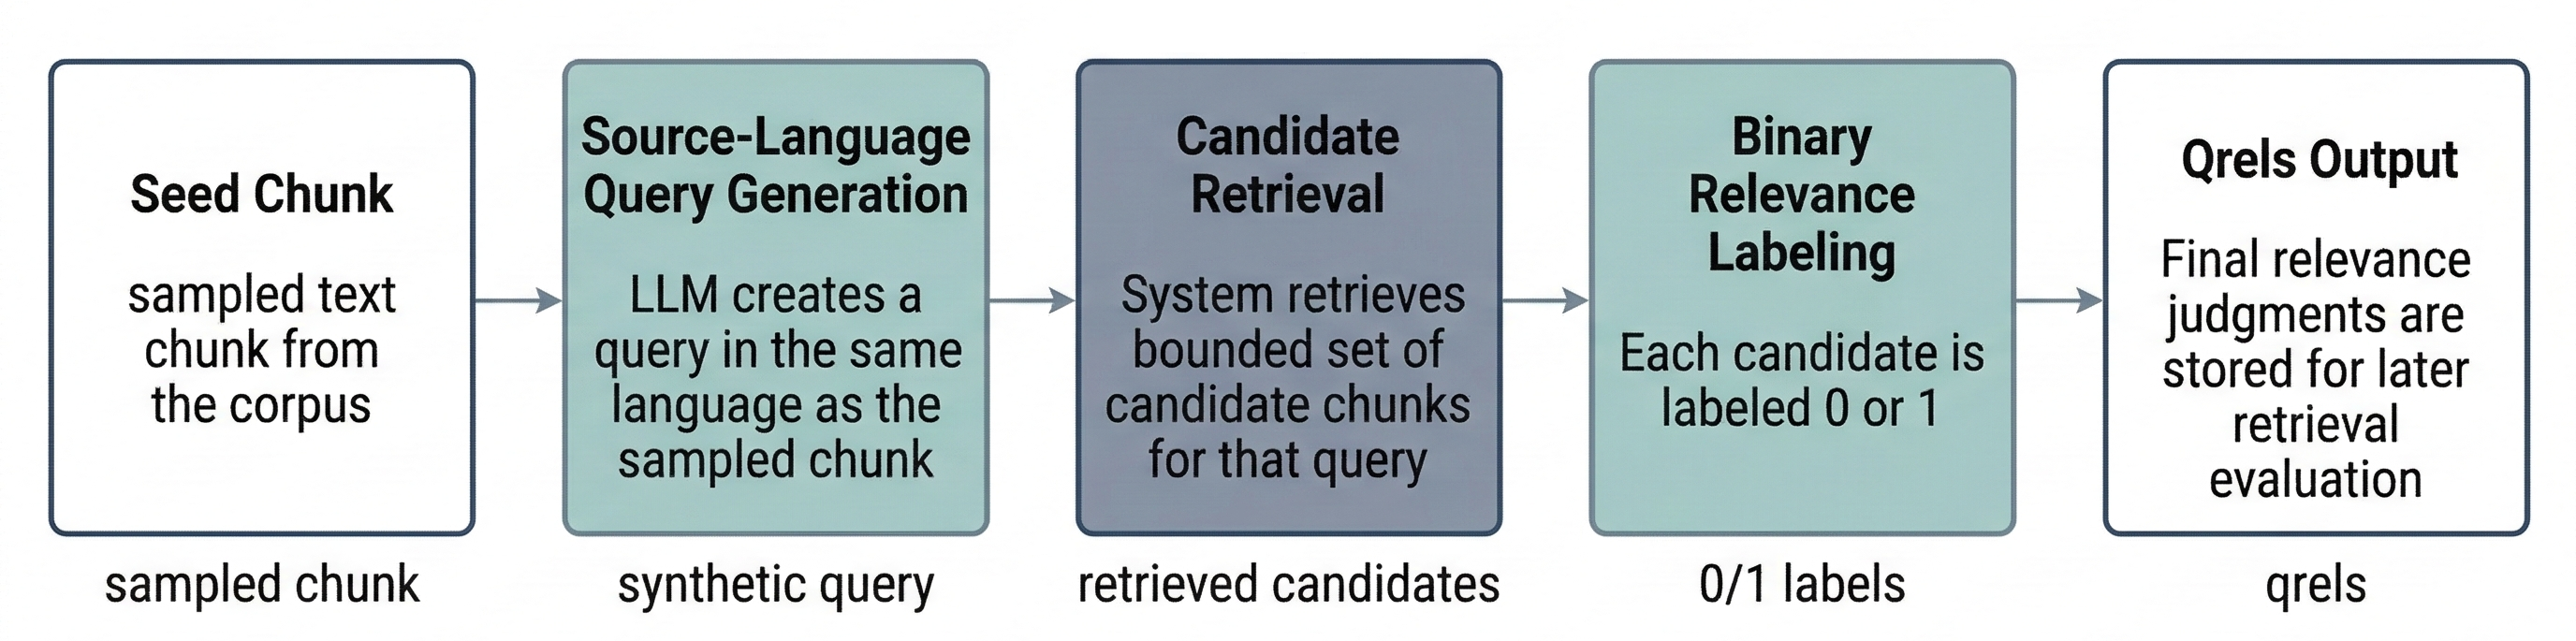
\includegraphics[width=0.95\linewidth]{query_qrels.png}
\caption{Workflow for synthetic query generation and binary relevance construction.}\label{fig:method_qrels_workflow}
\end{figure}

\subsection{Embedding Index Construction}\label{embedding-index-construction}

The comparative evaluation stage uses a fixed set of sentence-transformer models spanning lightweight, higher-capacity, and multilingual alternatives within a single benchmarking design. Each model is assigned its own vector collection so that embedding generation, storage, and retrieval remain isolated across models. This separation is methodologically important because it ensures that observed differences arise from the embedding models themselves rather than from shared or overwritten index state. The exact benchmarked model roster is specified in the experimental setup. \citep{SentenceTransformers_Pretrained}

Model-specific collections are built from the same chunked corpus. This means that corpus content, query set, and relevance judgments remain fixed while only the embedding function changes across runs. Such control is necessary if the benchmark is to support fit-for-purpose model selection rather than confound model comparison with changes in the evaluation dataset itself.

\subsection{Retrieval Evaluation Workflow}\label{retrieval-evaluation-workflow}

Once the vector collections are initialized, the pipeline executes the retrieval loop shown in Figure~\ref{fig:method_retrieval_workflow}. Each evaluation instance begins with a synthetic query drawn from the shared benchmark set. That query is submitted to a model-specific ChromaDB collection, where the embedding model under evaluation determines the vector representation used for search. The system then returns a ranked list of retrieved chunks under a fixed cutoff, ensuring that every model is tested at the same retrieval depth. The shared evaluation settings that constrain this loop are summarized in Section~\ref{shared-evaluation-setup}. \citep{ChromaDB_Docs}

The ranked results are subsequently aligned with the previously constructed qrels so that each query is interpreted against the same binary relevance resource, regardless of which embedding model produced the ranking. This ordering is methodologically important because corpus segmentation, query construction, and relevance judgments are all fixed before comparative retrieval begins. In combination with collection reinitialization, this design isolates representation quality from changes in benchmark artifacts or index state, allowing observed differences to be attributed more directly to the interaction between the candidate embedding model and the corpus.

The retrieval stage produces two classes of outputs. First, it emits evaluation-ready ranking artifacts that can be used in later scoring and comparative analysis. Second, it records timing traces associated with retrieval execution, thereby preserving operational evidence alongside effectiveness-oriented outputs. These timing by-products do not alter the retrieval protocol itself, but they allow the benchmark to support practical model selection under a single controlled workflow.

\begin{figure}
\centering
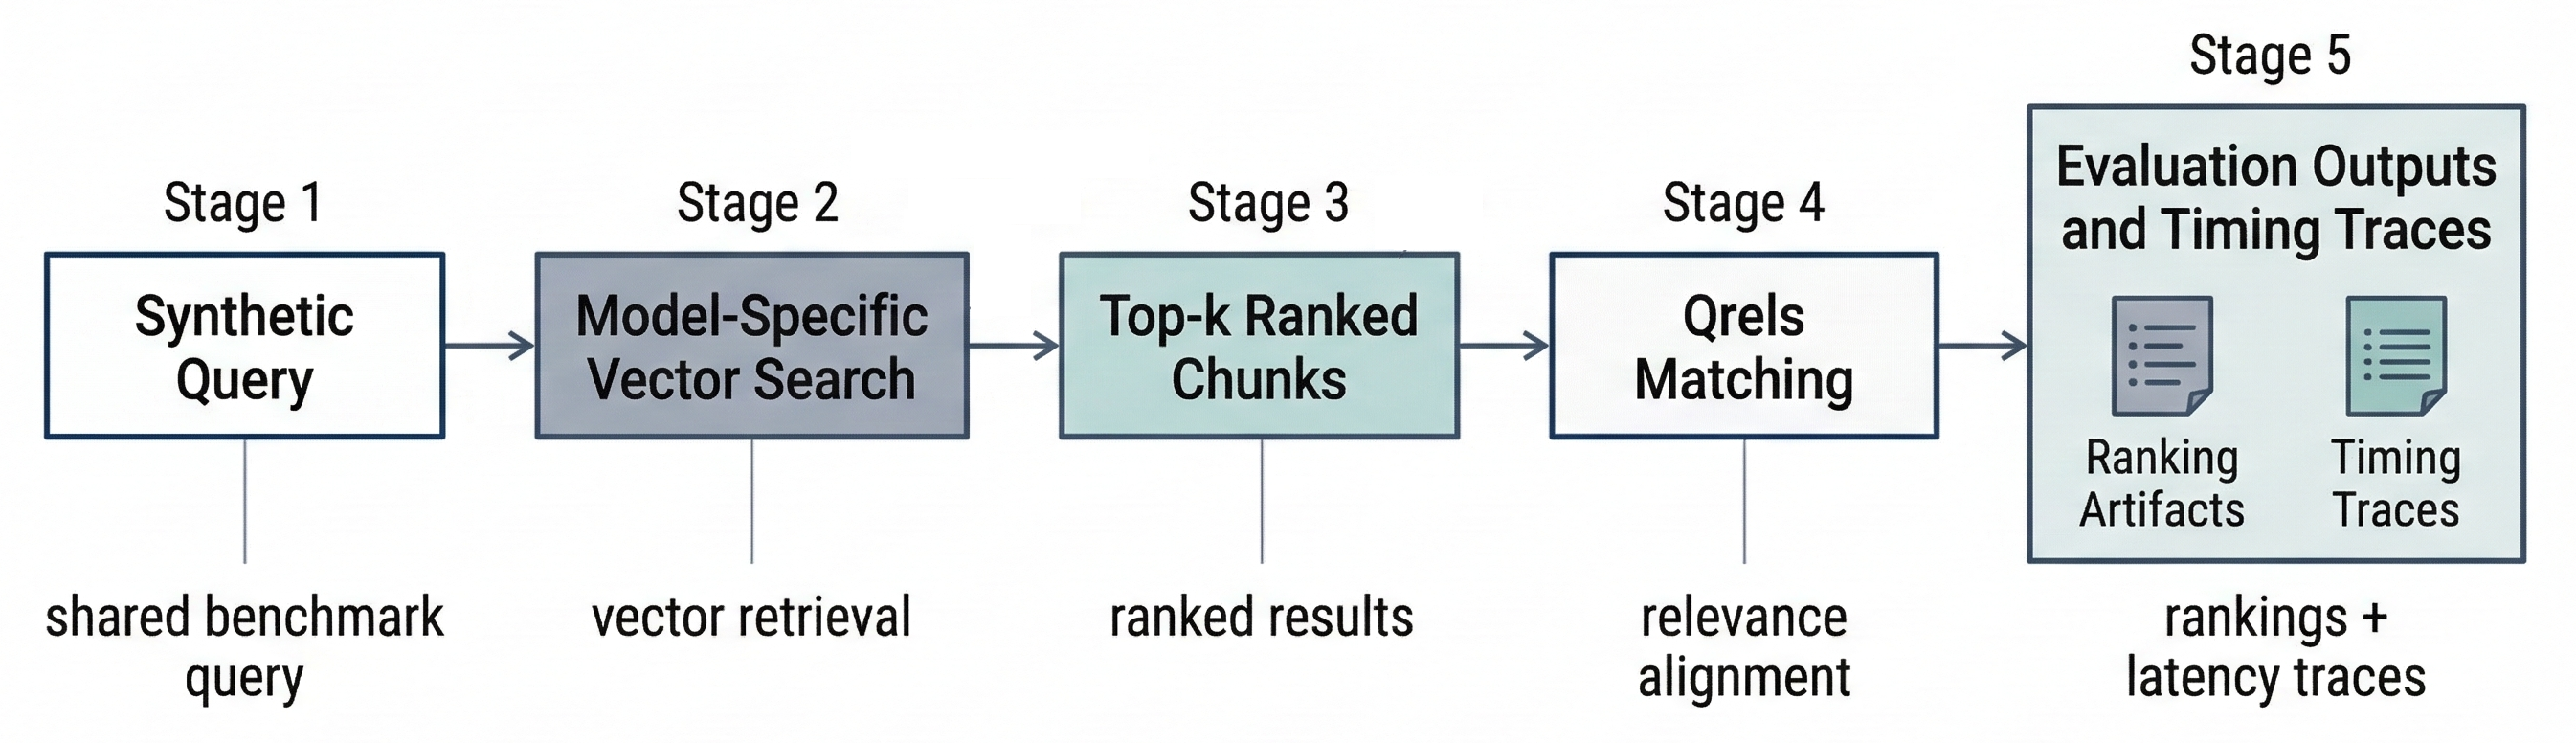
\includegraphics[width=0.95\linewidth]{evaluation_workflow.png}
\caption{Retrieval evaluation workflow from model-specific vector search to evaluation-ready ranking artifacts.}\label{fig:method_retrieval_workflow}
\end{figure}

\subsection{Automated Reporting and Reproducibility}\label{automated-reporting-and-reproducibility}

The final stage transforms raw benchmark outputs into structured reporting artifacts intended for comparative analysis and engineering reuse. As illustrated in Figure~\ref{fig:method_reporting_workflow}, this workflow is organized in two reporting layers whose outputs are summarized in Table~\ref{tbl:method_reporting_outputs}. The first layer operates separately for each dataset or dataset subset. When the objective is to select a suitable embedding model for one available corpus, or for a representative sample drawn from that corpus, the pipeline can terminate at this stage and produce a single benchmark report together with ranking summaries, timing summaries, and dataset-specific visualizations. These per-dataset artifacts preserve the full evaluation trace for one corpus under the shared model roster and provide a self-contained basis for model selection within that local context.

The second layer begins only after one or more dataset-level reports have been completed. This aggregation stage is intended for settings in which the available collection is heterogeneous, for example when documents belong to different topic classes such as finance, law, or administration, or when the corpus spans multiple languages such as English, Turkish, or French. In such cases, separate benchmark reports can be generated for the relevant subsets and then combined into an aggregate comparison package, as shown in Figure~\ref{fig:method_reporting_workflow}. The aggregate report is therefore derived from completed benchmark products rather than from raw retrieval outputs, which enables automatic inspection of how corpus variation affects embedding behavior across multiple evaluation criteria. The concrete experimental configuration and the resulting comparative evidence are presented in Sections~\ref{experiments} and~\ref{results}, respectively.

\begin{table}[t]
\caption{Reporting outputs produced by the proposed benchmarking pipeline.}\label{tbl:method_reporting_outputs}
\centering
\small
\begin{tabular}{@{}>{\raggedright\arraybackslash}p{0.16\linewidth}>{\raggedright\arraybackslash}p{0.36\linewidth}>{\raggedright\arraybackslash}p{0.36\linewidth}@{}}
\toprule
Output level & Artifacts & Purpose \\
\midrule
Dataset level & Benchmark report, ranking summaries, timing summaries, and dataset-specific visualizations & Support model selection for one corpus, one subset, or one representative sample under the shared model set \\
Aggregate level & Cross-dataset comparison report and comparative visual summaries & Consolidate heterogeneous dataset-level outputs into a reusable comparison package for cross-corpus or cross-subset inspection \\
\bottomrule
\end{tabular}
\end{table}

\begin{figure}
\centering
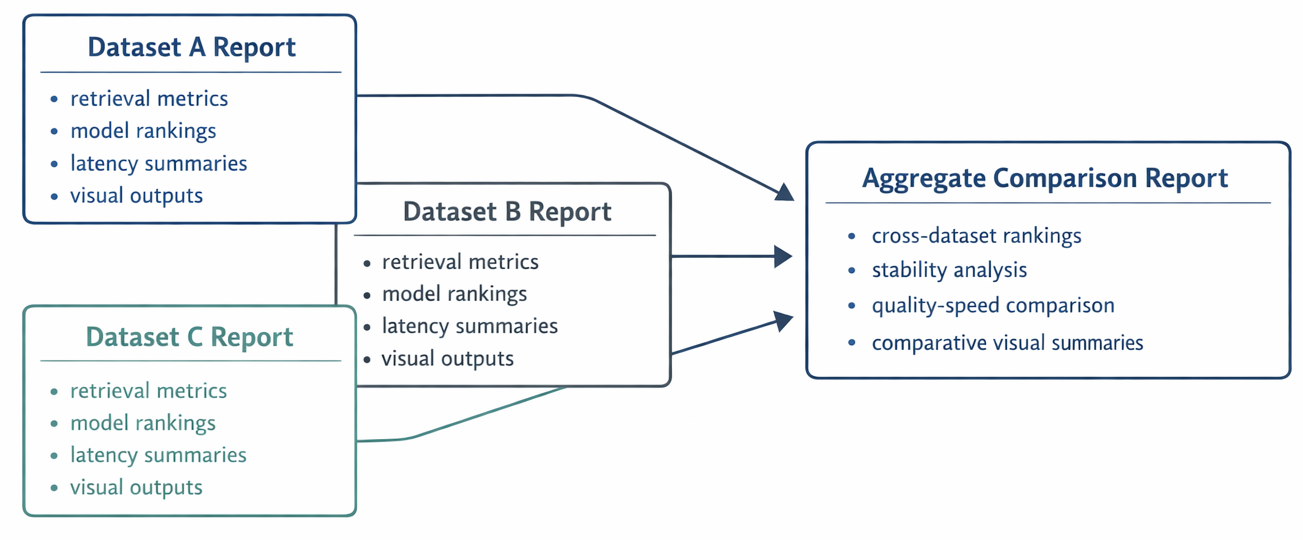
\includegraphics[width=0.95\linewidth]{report_generation.png}
\caption{Reporting flow from dataset-specific benchmark outputs to aggregate comparison artifacts.}\label{fig:method_reporting_workflow}
\end{figure}

The method is designed for reproducibility at both the artifact and workflow levels. Intermediate benchmark resources are materialized as explicit corpus, query, qrels, and report artifacts; model evaluation is performed on isolated vector collections; and reporting outputs are stored as timestamped run products at both dataset and aggregate levels. The implementation of this pipeline is publicly available for inspection and reuse, which supports transparent reconstruction of the benchmarking workflow described in this paper. \citep{GitHub_RagRetrievalBench}
